\documentclass[letterpaper]{article} %único necesario para: crear documento, hacer título, espacios, interlineado

\usepackage{vmargin} %necesario para ajustar las márgenes con \setmargins
\usepackage{euler} %usa la fuente "euler" para las ecuaciones
\usepackage{amsfonts} %para Z estilizada
\usepackage{pifont} %para más estilos de viñetas
\usepackage{amsmath} %necesario para equation*
\usepackage{graphicx} %para manejar imágenes
\usepackage{wrapfig} %para imágenes en modo "wrap"
\usepackage{lipsum} %para usar el texto de relleno
\graphicspath{ {./Images/} } %la dirección de la cual se sacan las imágenes

%letterpaper: 21.59cm x 27.94cm
\setmargins{1.5 cm} %margen izquierdo
{1.5 cm} %margen Superior
{17.5 cm} %anchura del texto
{25cm} %altura del texto
{0pt} %altura de los encabezados
{0cm} %espacio entre el texto y los encabezados
{0pt} %altura del pie de página
{0 cm} %espacio entre el texto y el pie de página


\pagenumbering{gobble} %Quita la numeración de las páginas
\renewcommand{\baselinestretch}{1} %Aumenta el interlineado a n veces el automático

\title{
  \textsc{
    \Large{Universidad Nacional de Colombia\\ Departamento de Matemáticas}\\ \vspace{0.1cm} 
    \large{Sistemas Numéricos}\\ \vspace{-0.1cm}
    \large{Examen 1 (II-2017) \hspace{1cm} Prof. José L. Ramírez}
  }
}

\date{}

\begin{document}
  
  \maketitle
  \vspace{-1cm}
  Nombre:\makebox[7cm]{\dotfill} Código:\makebox[3cm]{\dotfill} Fecha:\dotfill

  \vspace{0.5cm}
  
  \begin{itemize}
    
    \item[1.] Sea $\mathbb{Z}$ el conjunto de los números enteros.

      \begin{itemize}
      \item[\tiny{\ding{110}}] (\underline{0.5}) Demuestre que $\left( \mathbb{Z}, * \right)$, donde $a*b=a+b-1$ es un grupo abeliano.
      \item[\tiny{\ding{110}}] (\underline{0.5}) Demuestre que $\left( \mathbb{Z}, +\right)$ y $\left( \mathbb{Z}, *\right)$ son grupos isomorfos.
      \end{itemize}

    \item[2.] Sea $\left( G, *\right)$ un grupo. Definimos el conjunto $H_{G}:=\{h \in G: h'=h\}$.

      \begin{itemize}
      \item[\tiny{\ding{110}}] (\underline{0.5}) Demuestre que si $G$ es un grupo abeliano entonces $H_{G}$ es un subgrupo de $G$.
      \item[\tiny{\ding{110}}] (\underline{0.5}) Si la definición de $H_{G}$ se extiende para una estructura algebraica cualquiera, encuentre $H_{G}$ para $G=\left(\mathbb{Z}_{6}, \cdot \right)$.
      \end{itemize}

    \item[3.] (\underline{1.0}) Demostrar que si $m,n \in \mathbb{N}$ con $m<n$ entonces para todo número natural $p\neq0$,
      \begin{center}
        $mp<np$.
      \end{center}

    \item[4.] Considere la sucesión $\{P_{n} \}_{n\geq 0}$ definida por $P_{n}=2P_{n-1}+P_{n-2}$ para $n\geq 2$, con los valores iniciales $P_{0}=0$ y $P_{1}=1$.

      \begin{itemize}
      \item[\tiny{\ding{110}}] (\underline{0.5}) Demuestre que para todo número natural $n\geq 0$ se tiene que
      \begin{equation*}
        \sum_{k=0}^{n} P_{2k+1} = \frac{1}{2}P_{2n+2}.
      \end{equation*}
      \item[\tiny{\ding{110}}] (\underline{0.5}) Sea $Q_{n}$ el número de formas de teselar una cinta de tamaño $2\times n \left(n\geq 1\right)$ con las siguientes tres baldosas:\\

      \begin{center}
      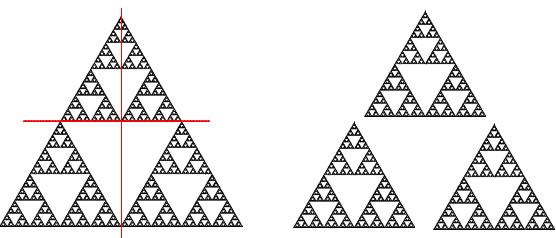
\includegraphics[height=2.5cm]{Fractal1} 
      \end{center}
      
      Demuestre que $Q_{n}=P_{n+1}$ para todo $n\geq 1$.
      \end{itemize}

    \item[5.] Sea $F_{n}$ el $n$-ésimo número de Fibonacci. Demuestre que $F_{n+1}<\left(\frac{7}{4}\right)^{n}$ para todo número natural $n\geq 1$.
        
  \end{itemize}
  
\end{document}
